%% Author_tex.tex
%% Template for Proc. R. Soc. A using rsproca_new.cls

\documentclass[openacc]{rsproca_new}%%%% where rsproca_new is the template name

%%%%%%%%%%% Defining Enunciations  %%%%%%%%%%%
\newtheorem{theorem}{\bf Theorem}[section]
\newtheorem{condition}{\bf Condition}[section]
\newtheorem{corollary}{\bf Corollary}[section]
%%%%%%%%%%%%%%%%%%%%%%%%%%%%%%%%%%%%%%%%%%%%%%%

%%%%% Article type %%%%%
\titlehead{Research}

\begin{document}

%%%% Article title %%%%
\title{Attentional Agents and Enactive Inference: A Computational Phenomenology of Mental Action}

%%%% Author details %%%%
\author{Prakash Chandra Kavi$^{1}$, Daniel Ari Friedman$^{2}$ and Gustavo Patow$^{1,3}$}

%%%% Author addresses %%%%
\address{
$^{1}$Universitat de Girona, Girona 17003, Spain\\
$^{2}$Active Inference Institute, Crescent City, CA 95531, USA\\
$^{3}$Universitat Pompeu Fabra, Barcelona 08002, Spain
}

%%%% Subject entries (Proc. R. Soc. A) %%%%
\subject{agency, computational modeling, mental simulations}

%%%% Keywords %%%%
\keywords{computational phenomenology, agency, active inference, attention, mental action, meditation}

%%%% Corresponding author %%%%
\corres{
Prakash Chandra Kavi\\
\email{prakash.kavi@gmail.com}
}

%%%% Abstract %%%%
\begin{abstract}
Meditative expertise involves sustained attention, rapid recovery from distraction, and coordinated dynamics of large‑scale brain networks. We present a computational phenomenology of focused‑attention meditation, characterizing transitions between four attractor states: breath focus, mind‑wandering, meta‑awareness, and redirection. We propose a hierarchical “russian doll” enactive inference architecture: (Layer‑1) a high‑dimensional neural substrate, modeled as a stochastic multivariate Ornstein–Uhlenbeck process capturing DMN, DAN, VAN, and FPN interactions; (Layer‑2) a low‑dimensional network of Markov‑blanketed attentional agents (“thoughtseeds”) that encode latent mental content and support policy evaluation; and (Layer‑3) a metacognitive monitor that modulates inference precision through content‑based meta‑awareness. In this formulation, meta‑awareness acts as a gain control on inference, while policy selection in Layer-2 minimizes expected free energy. Across expert vs. novice phenotypes, the model reproduces qualitative differences in dwell times, transition dynamics, and prediction errors that are consistent with contemplative neuroscience. The framework links first‑person phenomenology to mechanistic dynamics while remaining a minimal, mathematically tractable model of mental action.
\end{abstract}

\rsbreak

\maketitle

%%%%%%%%%% Main text starts here %%%%%%%%

\section{Introduction}
The neuroscientific investigation of meditation and mind-wandering has advanced considerably in recent years, providing valuable insights into attention regulation, metacognition, and the neural substrates of conscious experience \cite{BrandmeyerDelorme2021,Tang2015}. Meditative expertise is increasingly viewed as a self‑regulating process ‐ shaped by learned attentional strategies and network dynamics ‐ and is associated with enhanced cognitive flexibility, increased meta‑awareness and changes in interoceptive processing \cite{Dahl2015,Fox2014}. We  use focused-attention (FA) meditation, particularly Vipassana, as a tractable paradigm for modeling the “discursive mind”—the stream of internally generated thoughts, sensory impressions, and cognitive patterns similar to narrative ‐ that unfold over time \cite{Analayo2019}. Within this paradigm, we adopt a well‑established four‑stage attentional cycle during FA practice: breath focus, mind‑wandering, meta‑awareness (detection of mind‑wandering) and redirecting attention to breath \cite{Hasenkamp2012,Lutz2008}. From a neurocognitive perspective, this iterative cycle reflects the competitive and cooperative dynamics of large-scale brain networks \cite{ZamoraLopez2016}, aligning with predictive processing theories that frame cognition as the continuous minimization of prediction errors across scales \cite{BarrettSimmons2015,LaukkonenSlagter2021}. 

To formalize the self-regulating dynamics of meditative cognition, we adopt the Free Energy Principle (FEP), which posits that biological systems persist by minimizing variational free energy—an information-theoretic bound on surprise \cite{Friston2010}. This minimization is facilitated by a generative model that aligns internal predictions with sensory input through self-organizing perception-action loops \cite{ParrFriston2018}, where the statistical boundary—or Markov blanket—insulates an agent’s internal states while mediating its interactions with the environment \cite{Kirchhoff2018}. Within this framework, Active Inference provides the process theory for how “agents” enact free energy minimization through recurrent cycles of perception, learning, and action \cite{Friston2017,Ramstead2020}. By refining internal beliefs through perceptual inference and selecting policies that minimize expected free energy, agents effectively balance epistemic value (information gain) with pragmatic value (preferred outcomes) \cite{Friston2017}.

Physiologically, we ground these dynamics in the Neuronal Packet Hypothesis (NPH), which suggests that cognitive functions emerge from self-organizing ensembles of neurons called "neuronal packets" \cite{Yufik2019,YufikFriston2016,Ramstead2021}. These packets function as transient Markov blankets, enabling computational autonomy and conditional independence at various spatiotemporal scales \cite{Kirchhoff2018}, and can self-organize into higher order superordinate ensembles, to embody complex cognitive processes \cite{Ramstead2021}. This is further supported by the brain’s sparse architecture, which facilitates localized functional units \cite{SpornsBetzel2016}, forming hierarchical, nested Markov blanketed structures \cite{Hipolito2021}.The formation of superordinate ensembles reflects a hierarchical and heterarchical self-organization, where coordinated neuronal activity gives rise to emergent properties via a shared generative model \cite{Ramstead2021,Ramstead2022,Palacios2020}, such as the transient attentional states observed in meditation \cite{Hasenkamp2012}. These dynamics are shaped by internal precision estimates and are modulated through experience-dependent learning, such as meditation training \cite{Czajko2024,Hohwy2013,Varela2017}. 

We propose that discursive mental states could be characterized as emergent, functionally agentic entities. We operationalize these as "thoughtseeds" \cite{Kavi2025}—learned, low‑dimensional latent variables that act as subtle priors, biasing, and shaping high‑dimensional neural trajectories over time. These seeds are derived from underlying superordinate ensembles of neuronal packet dynamics \cite{Ramstead2021} via coarse-graining and a nucleation process, yielding compressed generative codes of latent mental impressions within their neuronal substrates. This formulation resonates with ālaya-vijñāna (storehouse consciousness), where mental "seeds" (bīja) persist as latent tendencies \cite{Analayo2019}. It aligns with "consciousness prior" which frames conscious content as a low-dimensional bottleneck \cite{Bengio2017} for the Global Neuronal Workspace (GNW) access \cite{Mashour2020,DehaeneChangeux2011} and with SOHM-style self-organization \cite{Safron2020}. Within this architectural bottleneck, thoughtseeds achieve agentic causation by providing compressed constraints that select, synchronize, and stabilize high-dimensional trajectories into coherent, resonant modes, thereby enabling tractable top-down shaping of cognitive dynamics.

To maintain both neurobiological relevance and computational tractability, our model focuses on the interaction between these agentic thoughtseeds and the four representative brain networks: Default Mode Network (DMN), Dorsal Attention Network (DAN), Ventral Attention Network (VAN) and Frontoparietal Network (FPN) \cite{Yeo2011}. We model meditation as a dynamic optimization process in which expertise is expressed through precision‑weighted competition among latent states. Adopting a computational phenomenology approach \cite{SandvedSmith2025,Ramstead2022,Varela2017} the model reproduces expert–novice differences in dwell times, transition profiles, and prediction errors, consistent with reported DMN suppression and accelerated distraction recovery \cite{Fox2015,Brewer2011,Dahl2015}. We characterize the four canonical stages of FA meditation \cite{Hasenkamp2012} as distinct attractor states within a hierarchical free-energy landscape \cite{Friston2014}.

\section{Materials and Methods}
\subsection{Conceptual Architecture and Simulation Strategy}
Drawing on Active Inference \cite{Friston2017} and Global Neuronal Workspace Theory \cite{Mashour2020,DehaeneChangeux2011}, the thoughtseeds framework's "russian doll architecture" is organized into a three-level nested Markov blanket hierarchy (see Fig.~\ref{fig_1}).

\begin{figure}[!h]
\centering
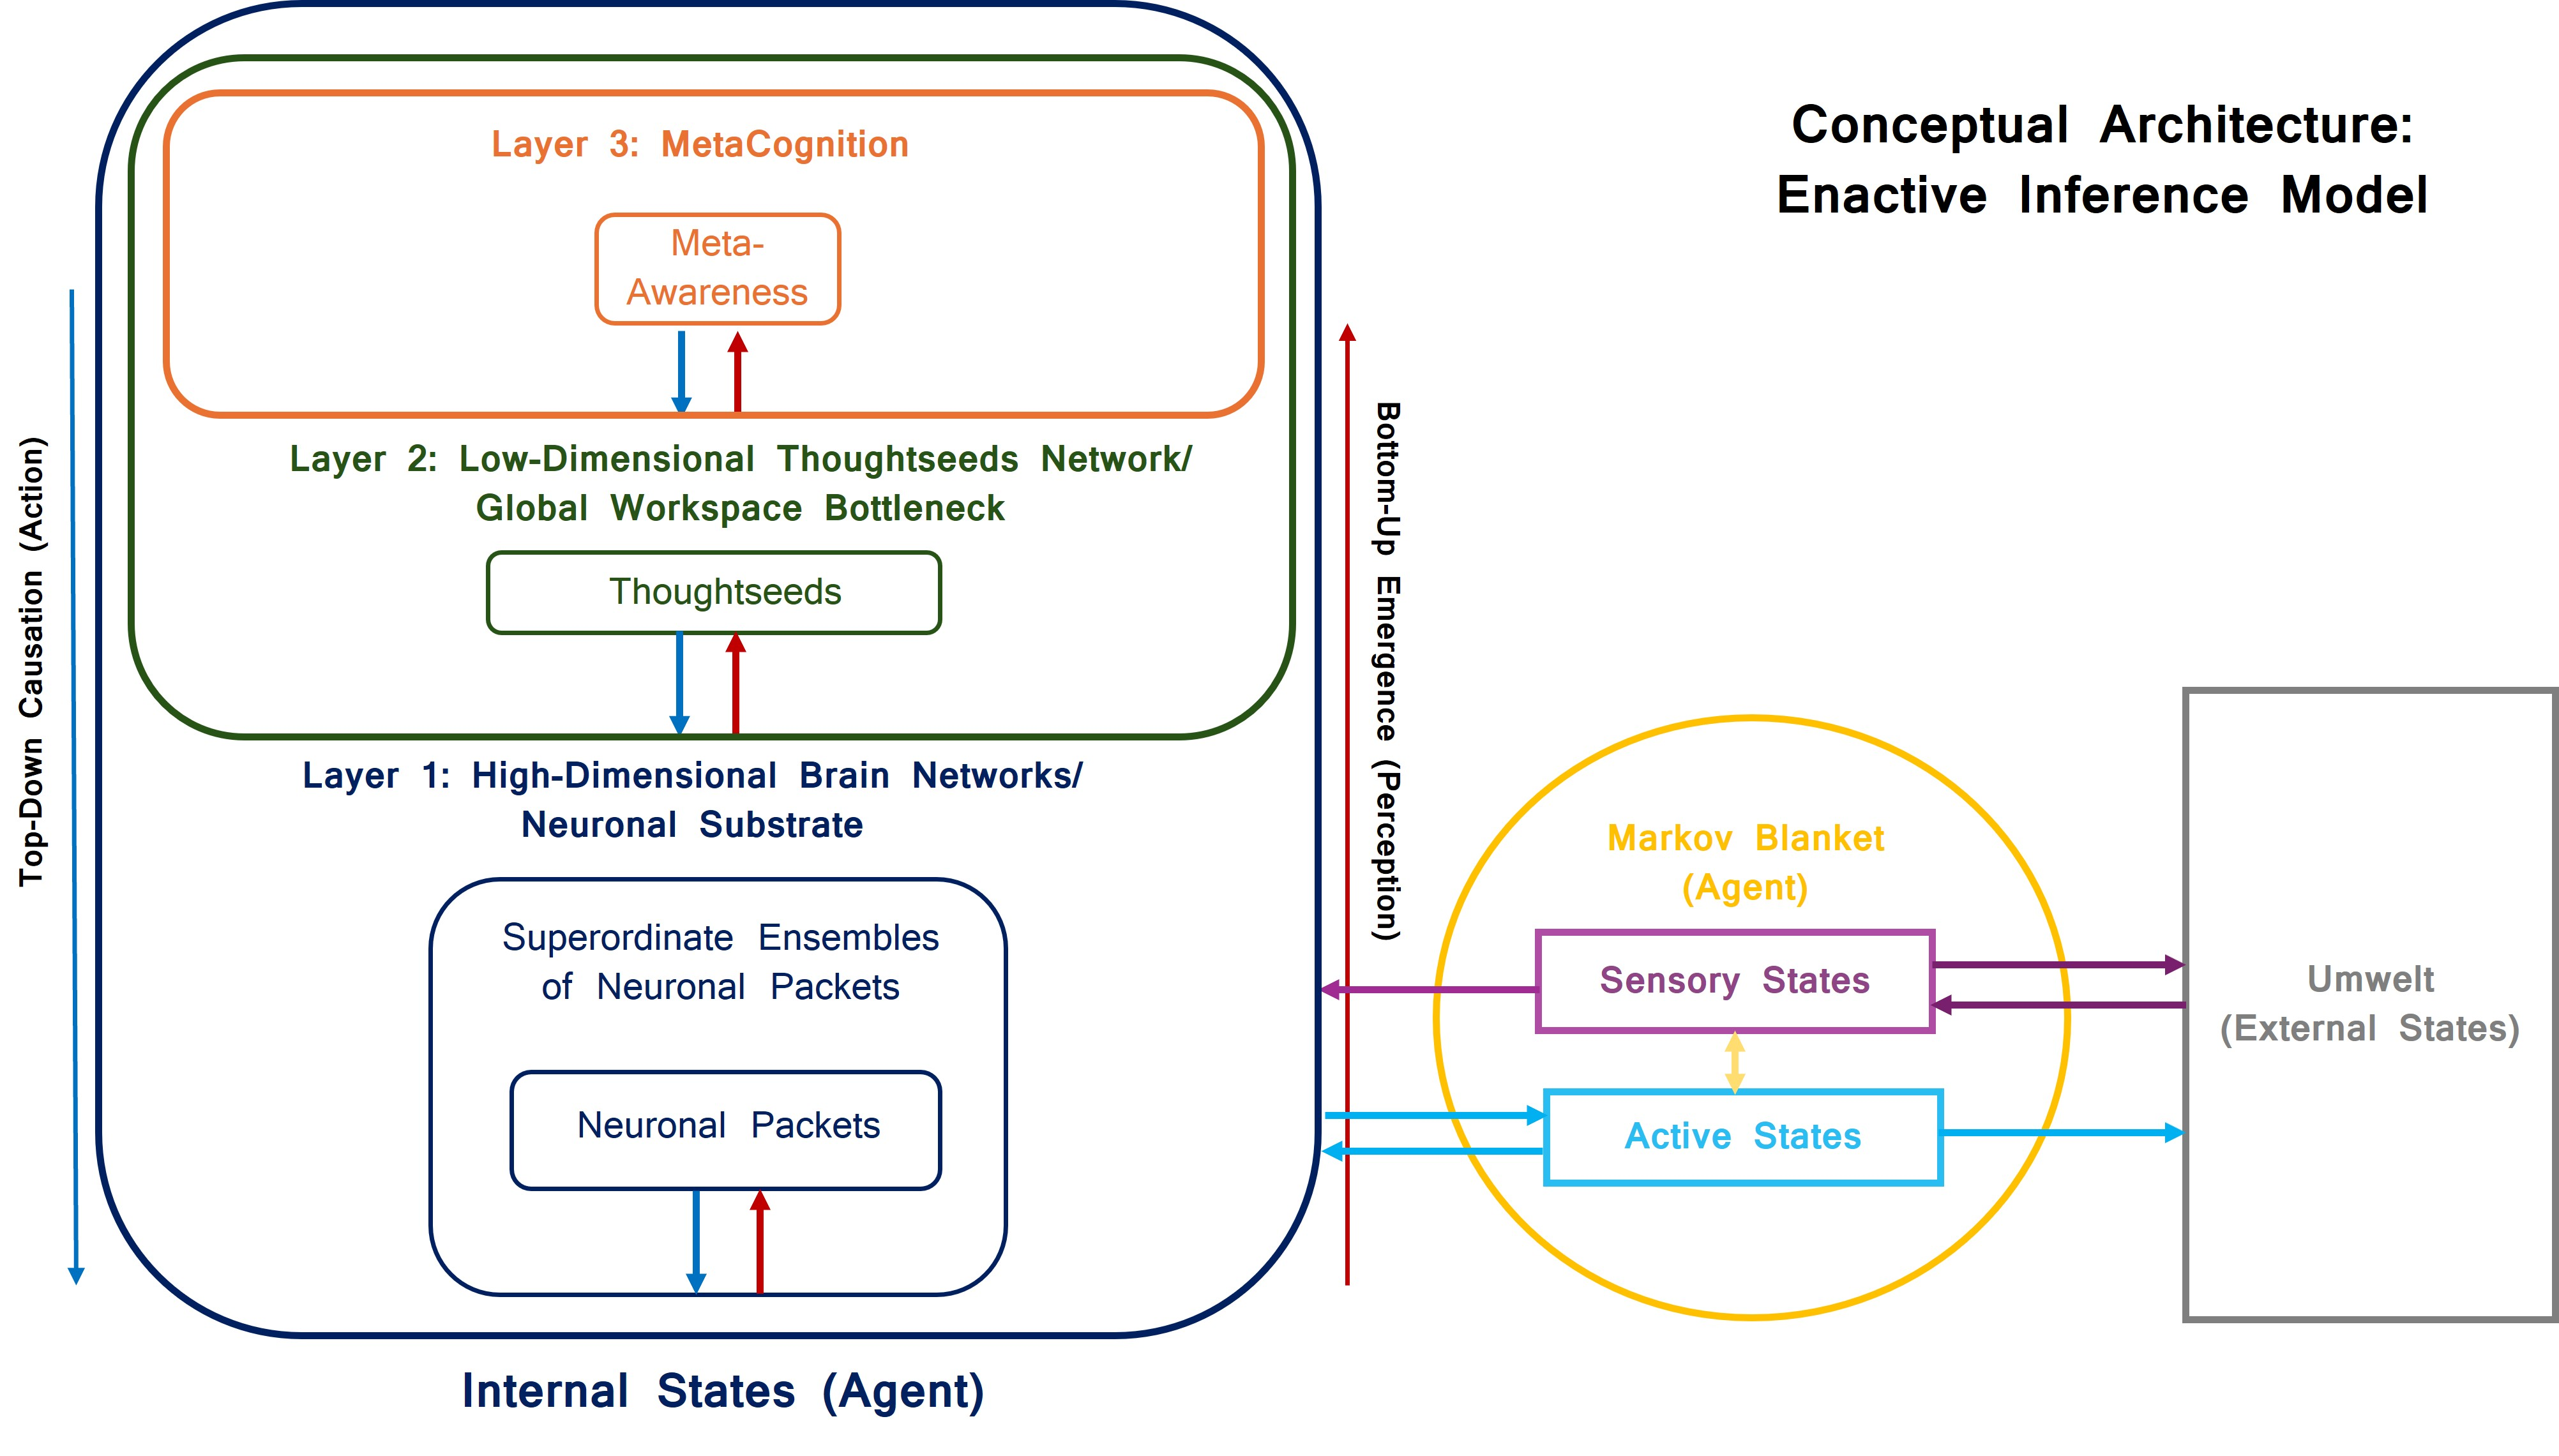
\includegraphics[width=\textwidth]{figures/fig1.png}
\caption{\textbf{Enactive Inference Model — Conceptual Architecture of Attentional Agents.}
\textbf{Layer-1: High-Dimensional Neural Substrate (Generative Process)}
This foundational layer represents the self-organization of neuronal packets into functional superordinate ensembles \cite{Yufik2019,Ramstead2021,Hipolito2021}. It provides the high-dimensional dynamical substrate of the model, grounded in large-scale brain networks for neurobiological grounding and model tractability \cite{Yeo2011}.
\textbf{Layer-2: Low-Dimensional Thoughtseeds Network (Generative Model of Mental Content)}
This layer instantiates a low-dimensional bottleneck consistent with the Consciousness Prior \cite{Bengio2017} operating within the Global Neuronal Workspace architecture \cite{Mashour2020}. Learned low-dimensional latent variables, termed ``thoughtseeds'', nucleate from Layer-1 dynamics through coarse-graining and function as subtle priors that bias high-dimensional neural trajectories \cite{Kavi2025}. The dominant thoughtseed emerges as the competitive winner within the GNW bottleneck, achieving agentic causation by imposing top-down constraints that stabilize neural activity into coherent attractor states corresponding to the four meditative stages in this simulation \cite{Mashour2020}. These thoughtseeds act as Markov-blanketed agents, each maintaining conditional independence while competing for workspace access and behavioral control \cite{Kirchhoff2018,Ramstead2021}.
\textbf{Layer-3: Metacognitive Monitor (Meta-awareness and Precision-Weighted Regulation)}
This layer computes content-based meta-awareness and regulates Layer-2 dynamics through precision modulation \cite{Hohwy2013,Friston2017}. This layer functions as the system's ``irreducible Markov blanket'', regulating access and gain without directly overwriting lower-level content \cite{Ramstead2023}.
\textbf{Information flow and Markov Blanket Interface}
The architecture implements enactive inference, where agents are constituted by the distinction between generative process (Layer-1 dynamics over neural states) and generative model (Layer-2 beliefs encoded by thoughtseeds) \cite{Ramstead2022}. Bidirectional hierarchical message passing enables this: bottom-up prediction errors (red arrows) ascend to update beliefs, while top-down predictions and precision-weighted priors (blue arrows) descend to constrain lower-layer dynamics \cite{ParrFriston2018}. Internal states are insulated by a Markov blanket that interfaces with the Umwelt through sensory and active states, instantiating the enactive cycle of perception and action \cite{Kirchhoff2018,Varela2017,Ramstead2020}.}

\label{fig_1}
\end{figure}

We present a minimal, testable simulation of this conceptual architecture rather than a full end‑to‑end Active Inference stack. Parameters are model assumptions informed by contemplative neuroscience of meditation, but they are not derived directly from neuroimaging. Implementation follows the three‑layer design: Layer-1 is a multivariate Ornstein–Uhlenbeck process \cite{Gilson2016}; Layer-2 is a variational auto‑encoder with a forward model that predicts the next‑step dynamics \cite{KingmaWelling2013}; Layer-3 computes meta‑awareness and modulates precision in L2. Policy inference is performed in L2 via the expected free energy using the model’s own predictions. This hybrid design is intentionally minimal, yet sufficient to realize the intended top‑down / bottom‑up structure of the conceptual architecture. 
 
\subsection{Mathematical Framework}

\subsubsection{State Spaces \& Dynamics}

We define four coupled state spaces:

\textbf{L1 network activations:} \( x_t \in [0,1]^4 \), as \(\{ \text{DMN}, \text{VAN}, \text{DAN}, \text{FPN} \}\). This is a deliberately low-dimensional proxy for large-scale and high-dimensional networks to keep the simulation tractable \cite{Yeo2011}.

\textbf{L2 thoughtseeds:} \( z_t \in [0,1]^5 \), as 
\(\{ \text{attend\_breath}, \text{pain\_discomfort},  \text{pending\_tasks}, \text{aha\_moment}, \\ \text{equanimity} \}\).

We used five latents as a low-dimensional bottleneck \cite{Miller1956,Bengio2017}.

\textbf{Meditation state:} \[s_t \in \{\mathrm{BF},\, \mathrm{MW},\, \mathrm{MA},\, \mathrm{RA}\}
\]
corresponding to the four‑stage attentional cycle \cite{Hasenkamp2012}.

\textbf{Policy: }\( \pi_t \) denotes the candidate state‑transition policies (stay or switch).

\vspace{1em}
\textbf{Layer‑1 (MVOU dynamics)} 
The neural substrate is modeled as a multivariate Ornstein–Uhlenbeck process, which captures noisy, mean‑reverting dynamics around a state‑dependent attractor:
\[
dx_t = -\Theta(s_t)\,\bigl(x_t - \mu_x(s_t)\bigr)\,dt + \sigma\, dW_t \tag{1}
\]

Here, \( \mu_x(s_t) \) is the state‑conditioned attractor profile (e.g., higher DMN during \(\mathrm{MW}\), and \( \Theta(s_t) \) sets the rate and direction of mean‑reversion. Concretely, \( \Theta(s_t) \) controls how quickly the network components return to their attractor and how strongly the networks inhibit or excite each other (e.g., DMN–DAN anticorrelation in \(\mathrm{BF}\)). Thus, a larger \( \Theta \) implies faster decay to the attractor, and off‑diagonal terms encode cross‑network coupling. The term \( \sigma\, dW_t \) is an isotropic process noise, with variance \(\sigma^2\).

\textbf{Layer‑2 (thoughtseed priors + forward dynamics)} 
Each meditation state provides a thoughtseed prior \( \mu_z(s_t) \) that acts as a target in latent space. A learned forward model \( f_\psi(x,z) \) predicts the next‑step network activation and provides the predictive signal used for policy evaluation and precision control.

\subsubsection{Inference \& Precision}

\textbf{Recognition \& reconstruction.} Layer‑2 uses a variational auto‑encoder (VAE). The encoder \(q_\phi(z \mid x)\) provides a fast amortized estimate of the latent thoughtseed state, while the decoder \(p_\theta(x \mid z)\) defines the likelihood over network activity. At each step, variational free energy is the sum of reconstruction surprisal and complexity:
\begin{equation}
F(z_t) = \underbrace{-\log p_\theta(x_t \mid z_t)}_{\text{reconstruction surprisal}}
+ \underbrace{D_{\mathrm{KL}}\big(q_\phi(z_t \mid x_t) \,\|\, p(z_t \mid s_t)\big)}_{\text{complexity}}
\tag{2}
\end{equation}
Reconstruction surprisal measures how unexpected the observed network state is under the decoder’s likelihood, and the KL term penalizes deviations from the state‑conditioned prior \(p(z_t \mid s_t)\equiv\mu_z(s_t)\).

\textbf{Fixed‑step Variational Inference.} The amortized posterior is refined by a small number of gradient steps, yielding a stable posterior \(z_t^*\) without a full inner optimization loop:
\begin{equation}
z \leftarrow z - \eta \nabla_z F(z) \tag{3}
\end{equation}
During training, the encoder is explicitly regularized to match this refined posterior, improving amortized inference by learning to approximate the variational optimum directly.

\textbf{Precision \& Meta-awareness.} The forward model predicts the next network state \(\hat{x}_t\). The inverse of the resulting prediction error is used to set sensory precision \(\lambda_{\mathrm{sens}}\):
\begin{equation}
\lambda_{\mathrm{sens}} = \frac{\sigma^2}{\sigma^2 + \lVert x_t - \hat{x}_t \rVert^2}
\tag{4}
\end{equation}
We fuse \(\lambda_{\mathrm{sens}}\) with meta‑awareness output \(m_t\) so that monitoring acts as a gain on inference confidence. This fused precision term sets the balance between encoder evidence (bottom-up) and the state‑conditioned prior (top-down) during variational inference.

\subsubsection{Policy Inference via Expected Free Energy}

\textbf{Policy set and dwell‑aware priors.}
At each step, the agent evaluates four candidate policies: remain in the current state or switch to one of the other three states. We use a quadratic dwell ramp to shift prior mass from staying to switching. Let \(d \in [0,1]\) be normalized dwell progress. Then
\[
h = d^2,\qquad
E(\text{stay}) = 1-h,\qquad
E(s') = h\,P(s' \mid s_t)
\tag{5}
\]
where \(P(s' \mid s_t)\) is the state‑dependent transition prior. Early in a dwell (\(d \approx 0\)), the prior favors staying; late in a dwell (\(d \approx 1\)), it favors switching.

\textbf{Expected free energy.}
Preferences are defined by the state‑conditioned target in network space,
\[
C_s = \mathrm{decode}(\mu_z(s)).
\]
For each candidate policy \(\pi \in \Pi\), we predict the next network state \(\hat{x}_\pi\) and compute expected free energy:
\begin{equation}
G(\pi) =
\underbrace{D_{\mathrm{KL}}\!\big(\hat{x}_\pi \,\|\, C_{s_\pi}\big)}_{\text{risk}}
+
\underbrace{H(\hat{x}_\pi)}_{\text{ambiguity}}
\tag{6}
\end{equation}
The first term (risk) penalizes deviation from preferred outcomes; the second term (ambiguity) penalizes uncertainty in predicted outcomes.

\textbf{Policy posterior and precision.}
The posterior over policies combines the dwell‑aware prior \(E(\pi)\) with expected free energy:
\begin{equation}
q(\pi) = \mathrm{softmax}\!\big(\log E(\pi) - \gamma\, G(\pi)\big),
\qquad
\gamma = 1 - \frac{H\!\left(q(\pi)\right)}{\log |\Pi|}.
\tag{7}
\end{equation}
Here \(\gamma\) is policy precision (lower entropy \(\Rightarrow\) higher precision).

\textbf{Policy‑weighted target.}
The selected latent target is the posterior‑weighted mixture of state‑conditioned priors,
\begin{equation}
\mu = \sum_{\pi} q(\pi)\, \mu_z(s_\pi), 
\qquad
\mu_x = \mathrm{decode}(\mu).
\tag{8}
\end{equation}
This decoded target \(\mu_x\) is passed to L1 as the action‑relevant constraint.

\subsubsection{Learning Objective}

Training minimizes a \textbf{composite loss function} that balances variational free energy, forward surprisal, and recognition consistency:
\[
L_t = F_t + w_{\mathrm{fwd}}\, S_{\mathrm{fwd},t} + \alpha_{\mathrm{rec}}\, L_{\mathrm{rec},t}
\tag{9}
\]
where \(F_t\) is variational free energy (Eq.~2), \(S_{\mathrm{fwd},t}\) is forward surprisal (Eq.~4), and
\(L_{\mathrm{rec},t} = \lVert \mathrm{encode}(x_t) - z_t^{*} \rVert^2\) aligns the encoder with the VI‑refined latent state.
The forward weight \(w_{\mathrm{fwd}}\) is computed as an EMA‑stabilized ratio between \(F_t\) and \(S_{\mathrm{fwd},t}\) to keep the forward term scale‑matched. Experts use full recognition loss (\(\alpha_{\mathrm{rec}}=1\)); novices use a weaker scale tied to learning rate.

\section{Simulation Results}

\subsection{Simulation Strategy and Parameters}

We simulate two phenotypes (novice, expert) under the same architecture and state space, differing in learning rate and recognition‑loss scaling (weak vs.\ strong amortization) as well as dwell ranges and transition priors specified in config.

\textbf{Protocol}  
Training horizon: 10{,}000 timesteps per phenotype (dt fixed in config).  
Tail window: last 2{,}000 steps used for plots/diagnostics (stable regime).  
BPTT: gradients accumulated in fixed‑length windows (50 steps).  
Random seed: fixed for reproducibility; stochastic transitions remain seed‑controlled.  
Outputs: full trajectories (states, networks, thoughtseeds), VFE, policy metrics, prediction errors, and plots.

\textbf{Core parameters (config‑driven)}  
L1: MVOU dynamics, state‑dependent coupling (THETA\_BASE), network profiles, and global noise (NOISE\_LEVEL).  
L2: thoughtseed priors, encoder/decoder/forward model, fixed VI steps.  
L3: meta‑awareness weights; precision modulation in L2 only.  
Policies: dwell‑aware priors and softmax posteriors; precision from policy entropy.

This strategy is designed to be stable, reproducible, and interpretable while capturing expert–novice differences in dwell times, transitions, and prediction errors.

\subsection{Signatures of Attentional Expertise}

\subsubsection{Summary of Steady‑State Phenotypes}
Fig~\ref{fig_2} demonstrates diagnostic views of stabilised expert and novice profiles from the tail window.

\captionsetup{font=small}
\begin{figure*}[t!]
\centering
\begin{tabular}{c}
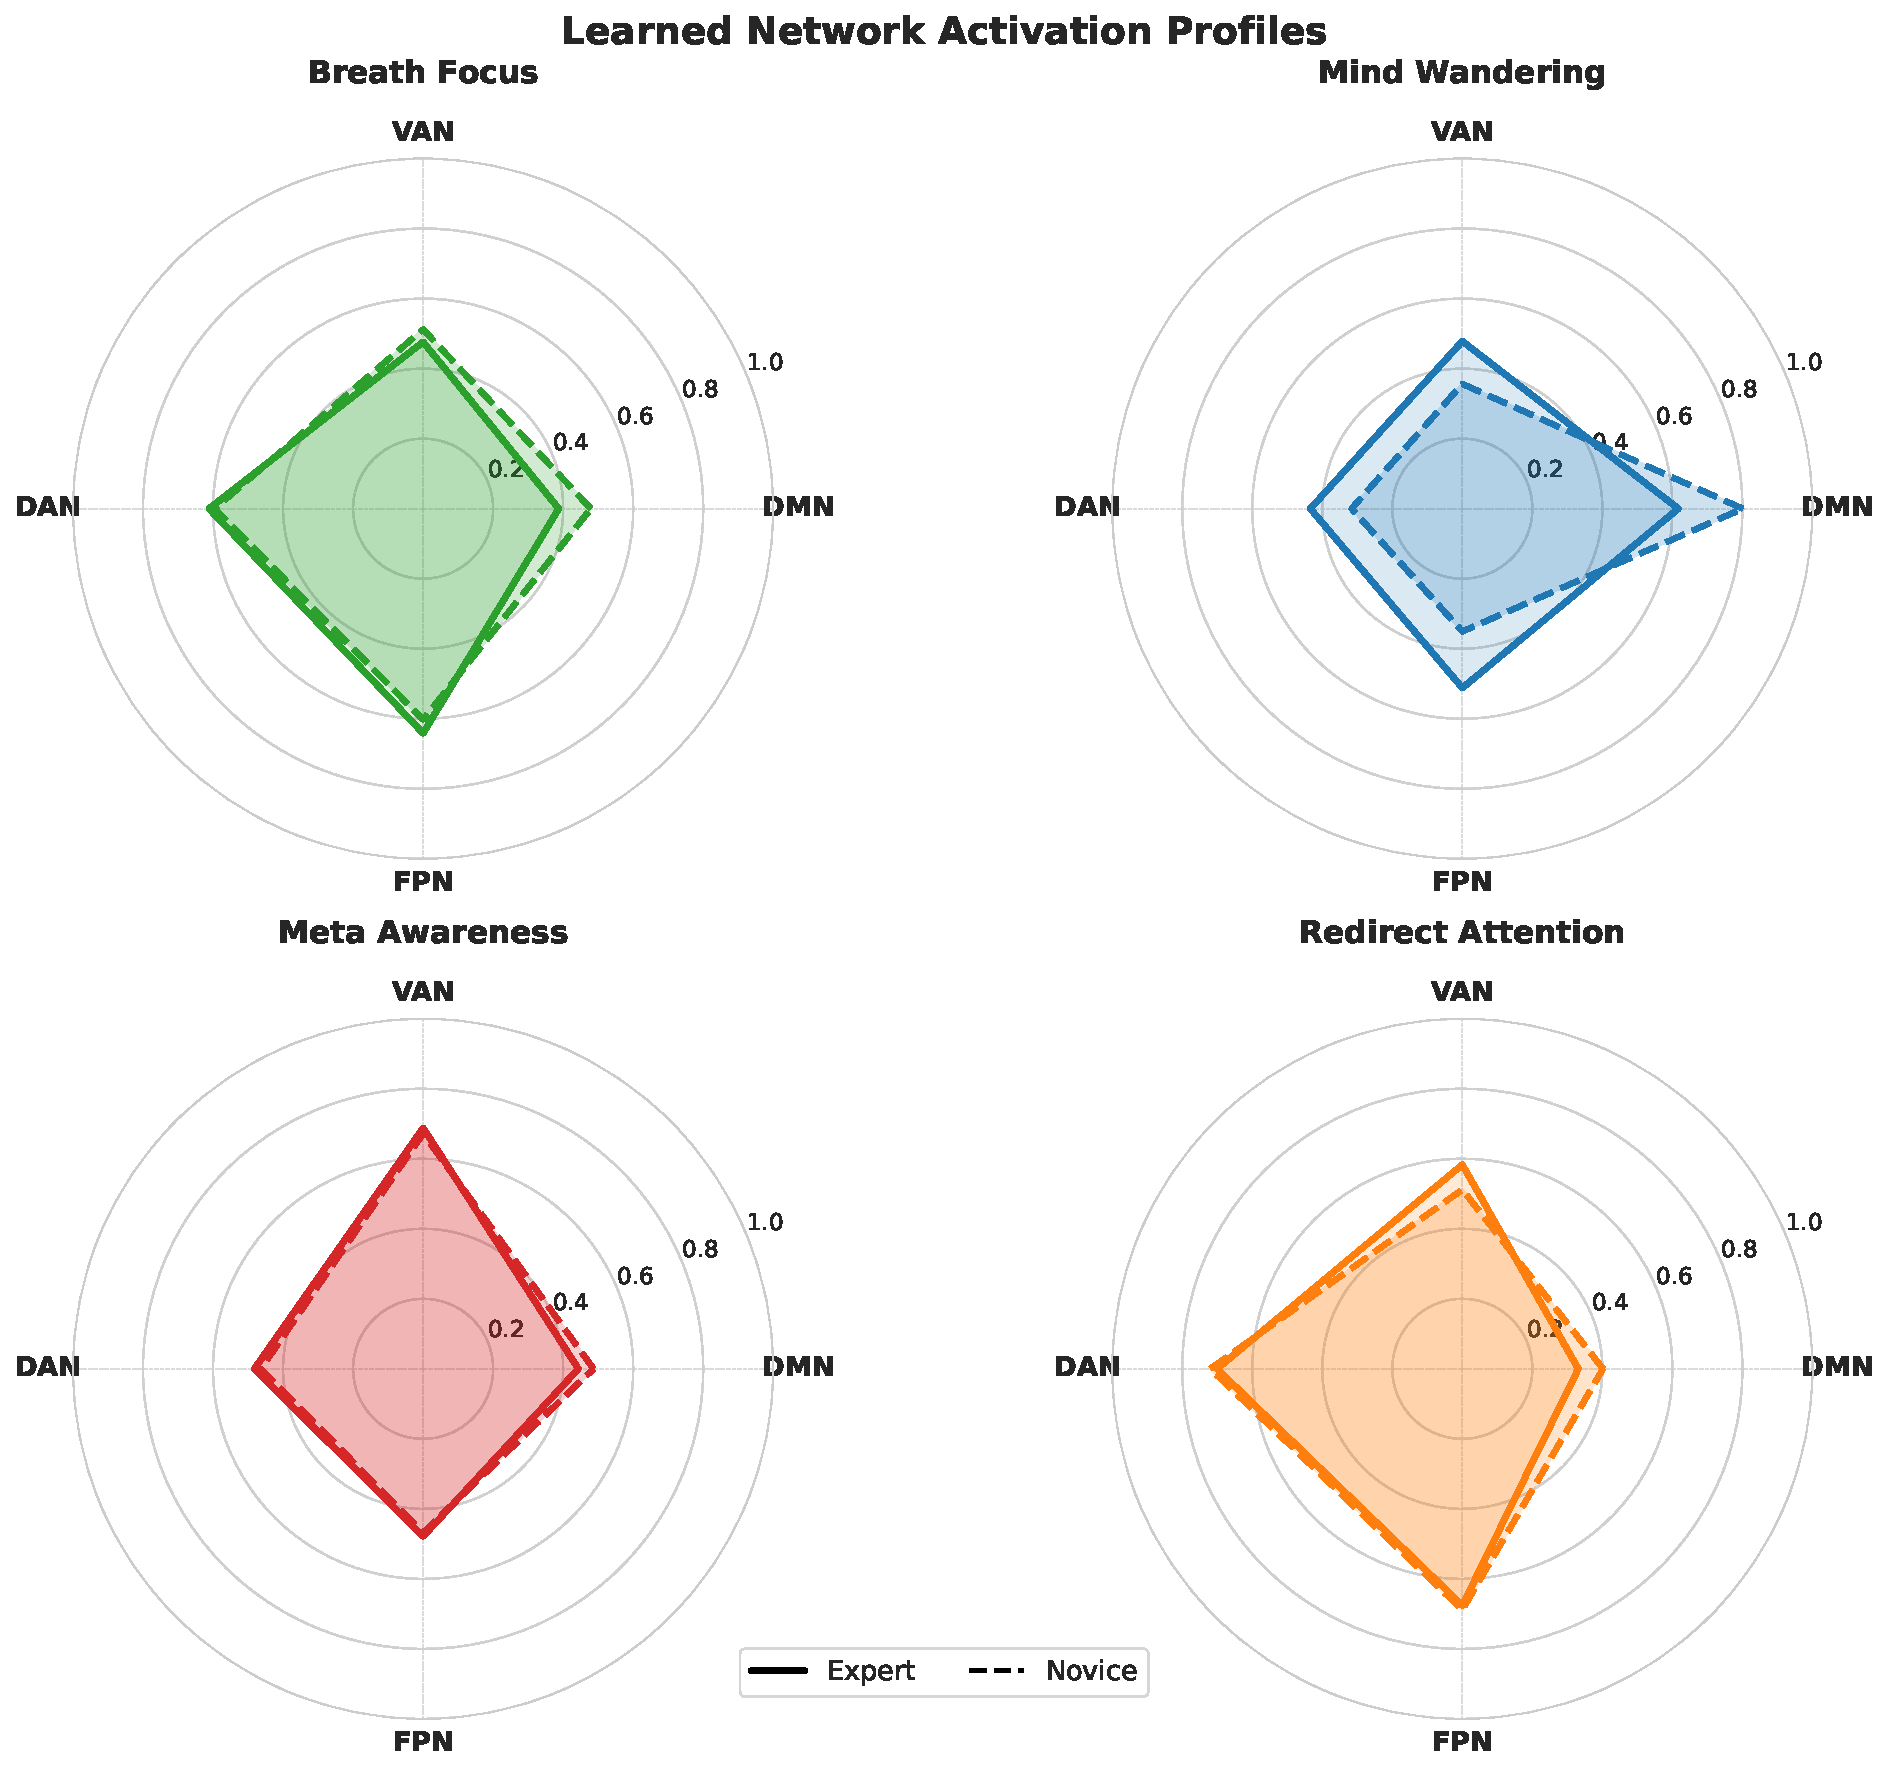
\includegraphics[width=0.9\textwidth]{figures/fig2a.pdf} \\
\small{(A)}
\end{tabular}
\vspace{0.5em}

\begin{tabular}{@{}c@{\hspace{0.5cm}}c@{}}
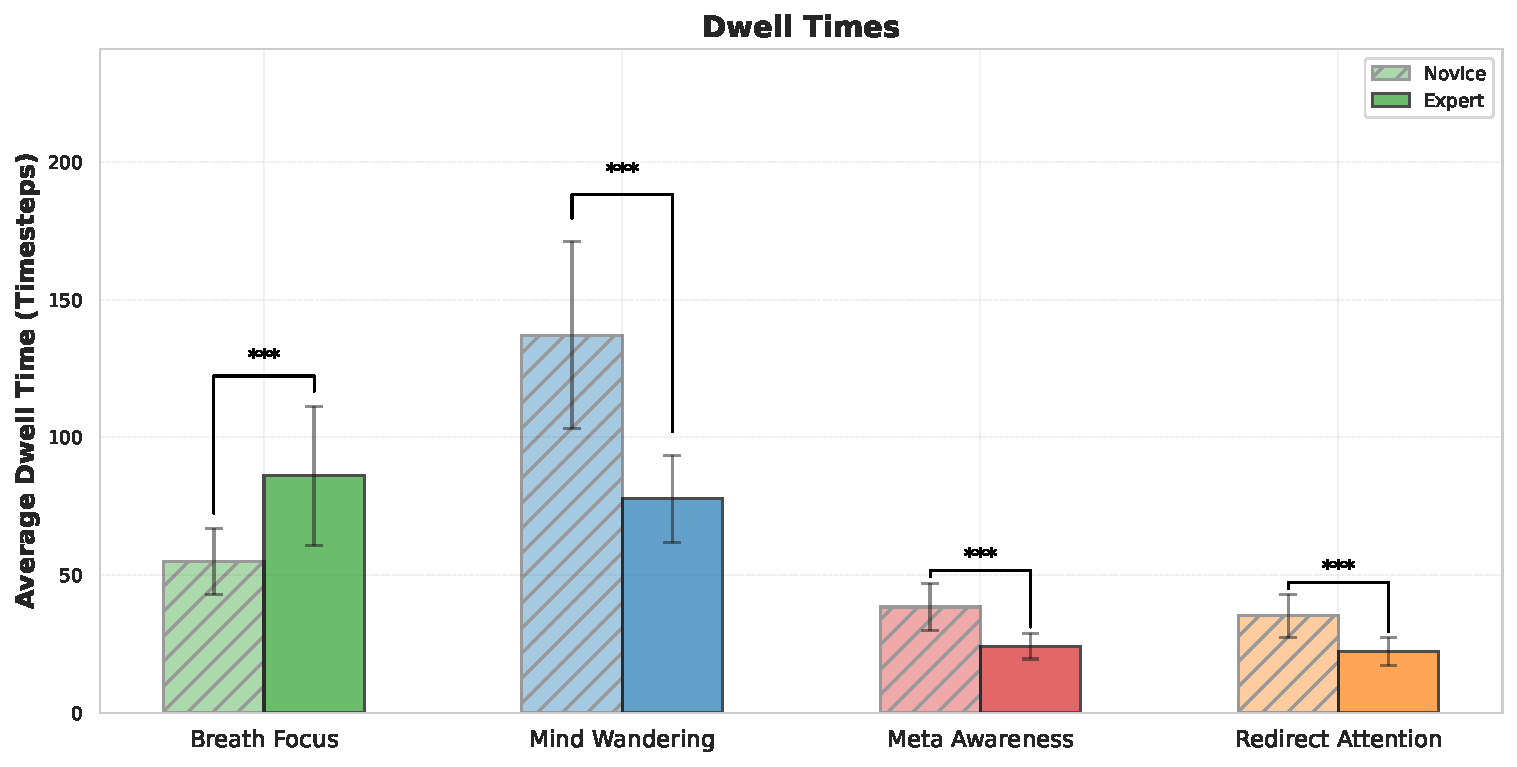
\includegraphics[width=0.45\textwidth]{figures/fig2b.pdf} &
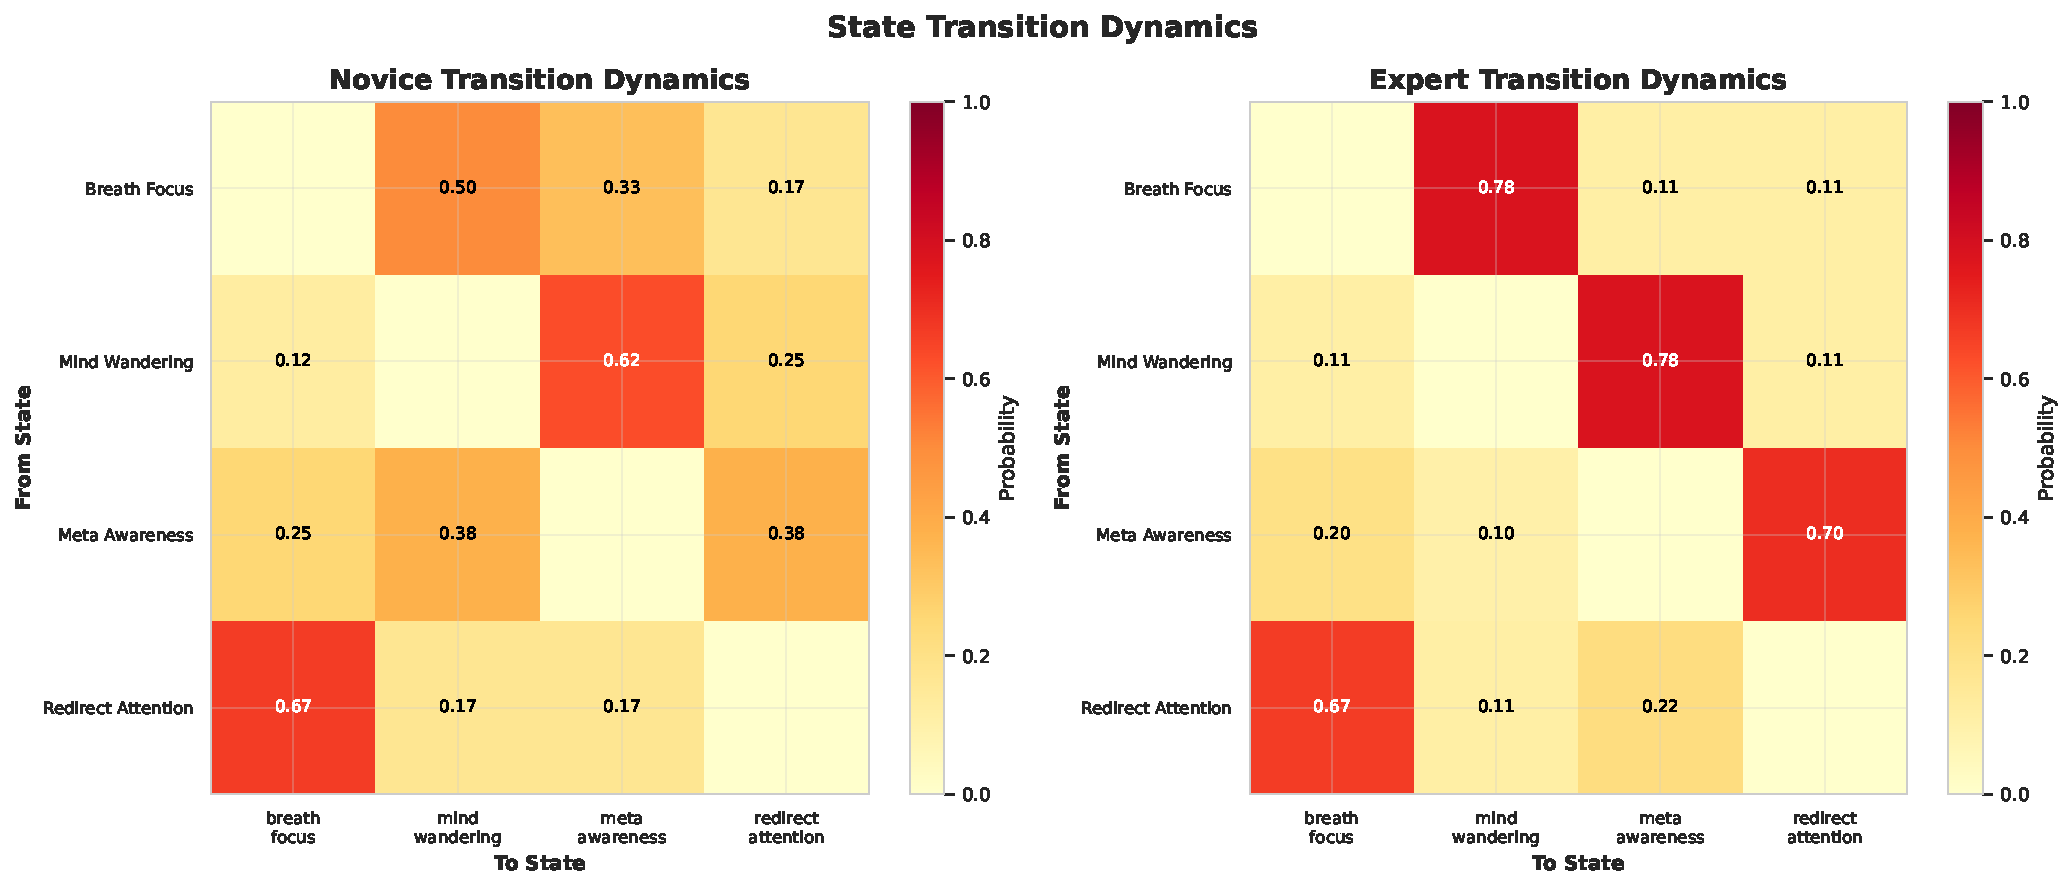
\includegraphics[width=0.45\textwidth]{figures/fig2c.pdf} \\
\small{(B)} & \small{(C)}
\end{tabular}
\caption{\textbf{Diagnostic Views of Stabilized Profiles.}
\textbf{(A) Network activation profiles.}
In Breath Focus, experts show stronger DMN suppression (0.39 vs 0.48) and higher control-network engagement (DAN 0.61, FPN 0.64) compared to novices (DAN 0.60, FPN 0.60), consistent with enhanced sustained attention and executive control from intensive meditation practice \cite{MacLean2010,Dahl2015}.
In Mind Wandering, novices show DMN-dominant profiles (0.80) while experts retain partial control-network engagement (DMN 0.62, DAN 0.43, FPN 0.51), echoing altered DMN activity and background monitoring in experienced practitioners \cite{Brewer2011,Fox2015}.
Meta-Awareness elevates VAN in both groups (expert 0.69, novice 0.67), consistent with salience-network recruitment during conscious detection of mind-wandering \cite{Hasenkamp2012,Seeley2007}.
During Redirect Attention, experts maintain lower DMN (0.33 vs 0.40) with strong DAN/FPN recruitment, reflecting more efficient re-engagement of task-positive networks in long-term meditators \cite{Lutz2008,Escrichs2019}.
Overall, experts exhibit lower DMN and higher control-network engagement across states, consistent with meditation-related shifts in default-mode and control-network balance \cite{Tang2015}.
\textbf{(B) Dwell times.}
Experts sustain Breath Focus longer (86.0 vs 55.0 steps) and remain in Mind Wandering far less (77.7 vs 137.1), matching findings that intensive training increases on-task time while reducing mind-wandering \cite{MacLean2010,Christoff2009,Dahl2015}.
Regulatory states are shorter for experts—Meta-Awareness (24.1 vs 38.4) and Redirect (22.2 vs 35.2)—consistent with earlier detection of mind-wandering and faster focus recovery in experienced meditators \cite{Hasenkamp2012,Lutz2008}.
This pattern reflects stronger focus maintenance, shorter lapses, and faster recovery, paralleling longitudinal effects of mindfulness training on attention and cognitive control \cite{Tang2015,Lutz2024}.
\textbf{(C) Transition dynamics.}
Experts show clearer recovery loops with higher MW$\rightarrow$MA transitions (0.78 vs 0.63) and stronger MA$\rightarrow$RA bias (0.70 vs 0.38), closely mirroring the canonical MW$\rightarrow$MA$\rightarrow$RA$\rightarrow$BF sequence identified in focused-attention meditation studies \cite{Hasenkamp2012,Lutz2008}.
Experts are less likely to cycle back into MW from MA (0.10 vs 0.38), consistent with meta-awareness more reliably leading to re-engagement in experienced practitioners \cite{Schooler2011,Fox2015}.
Novices show more diffuse transitions (MW$\rightarrow$RA = 0.25 vs 0.11), indicating less focused recovery.
The expert transition matrix concentrates probability on the canonical loop, while novice transitions are more distributed, capturing known differences between novice and expert meditation dynamics \cite{Dahl2015,Escrichs2019}.}
\label{fig_2}
\end{figure*}


\begin{figure*}[t!]
\centering
\begin{tabular}{c}
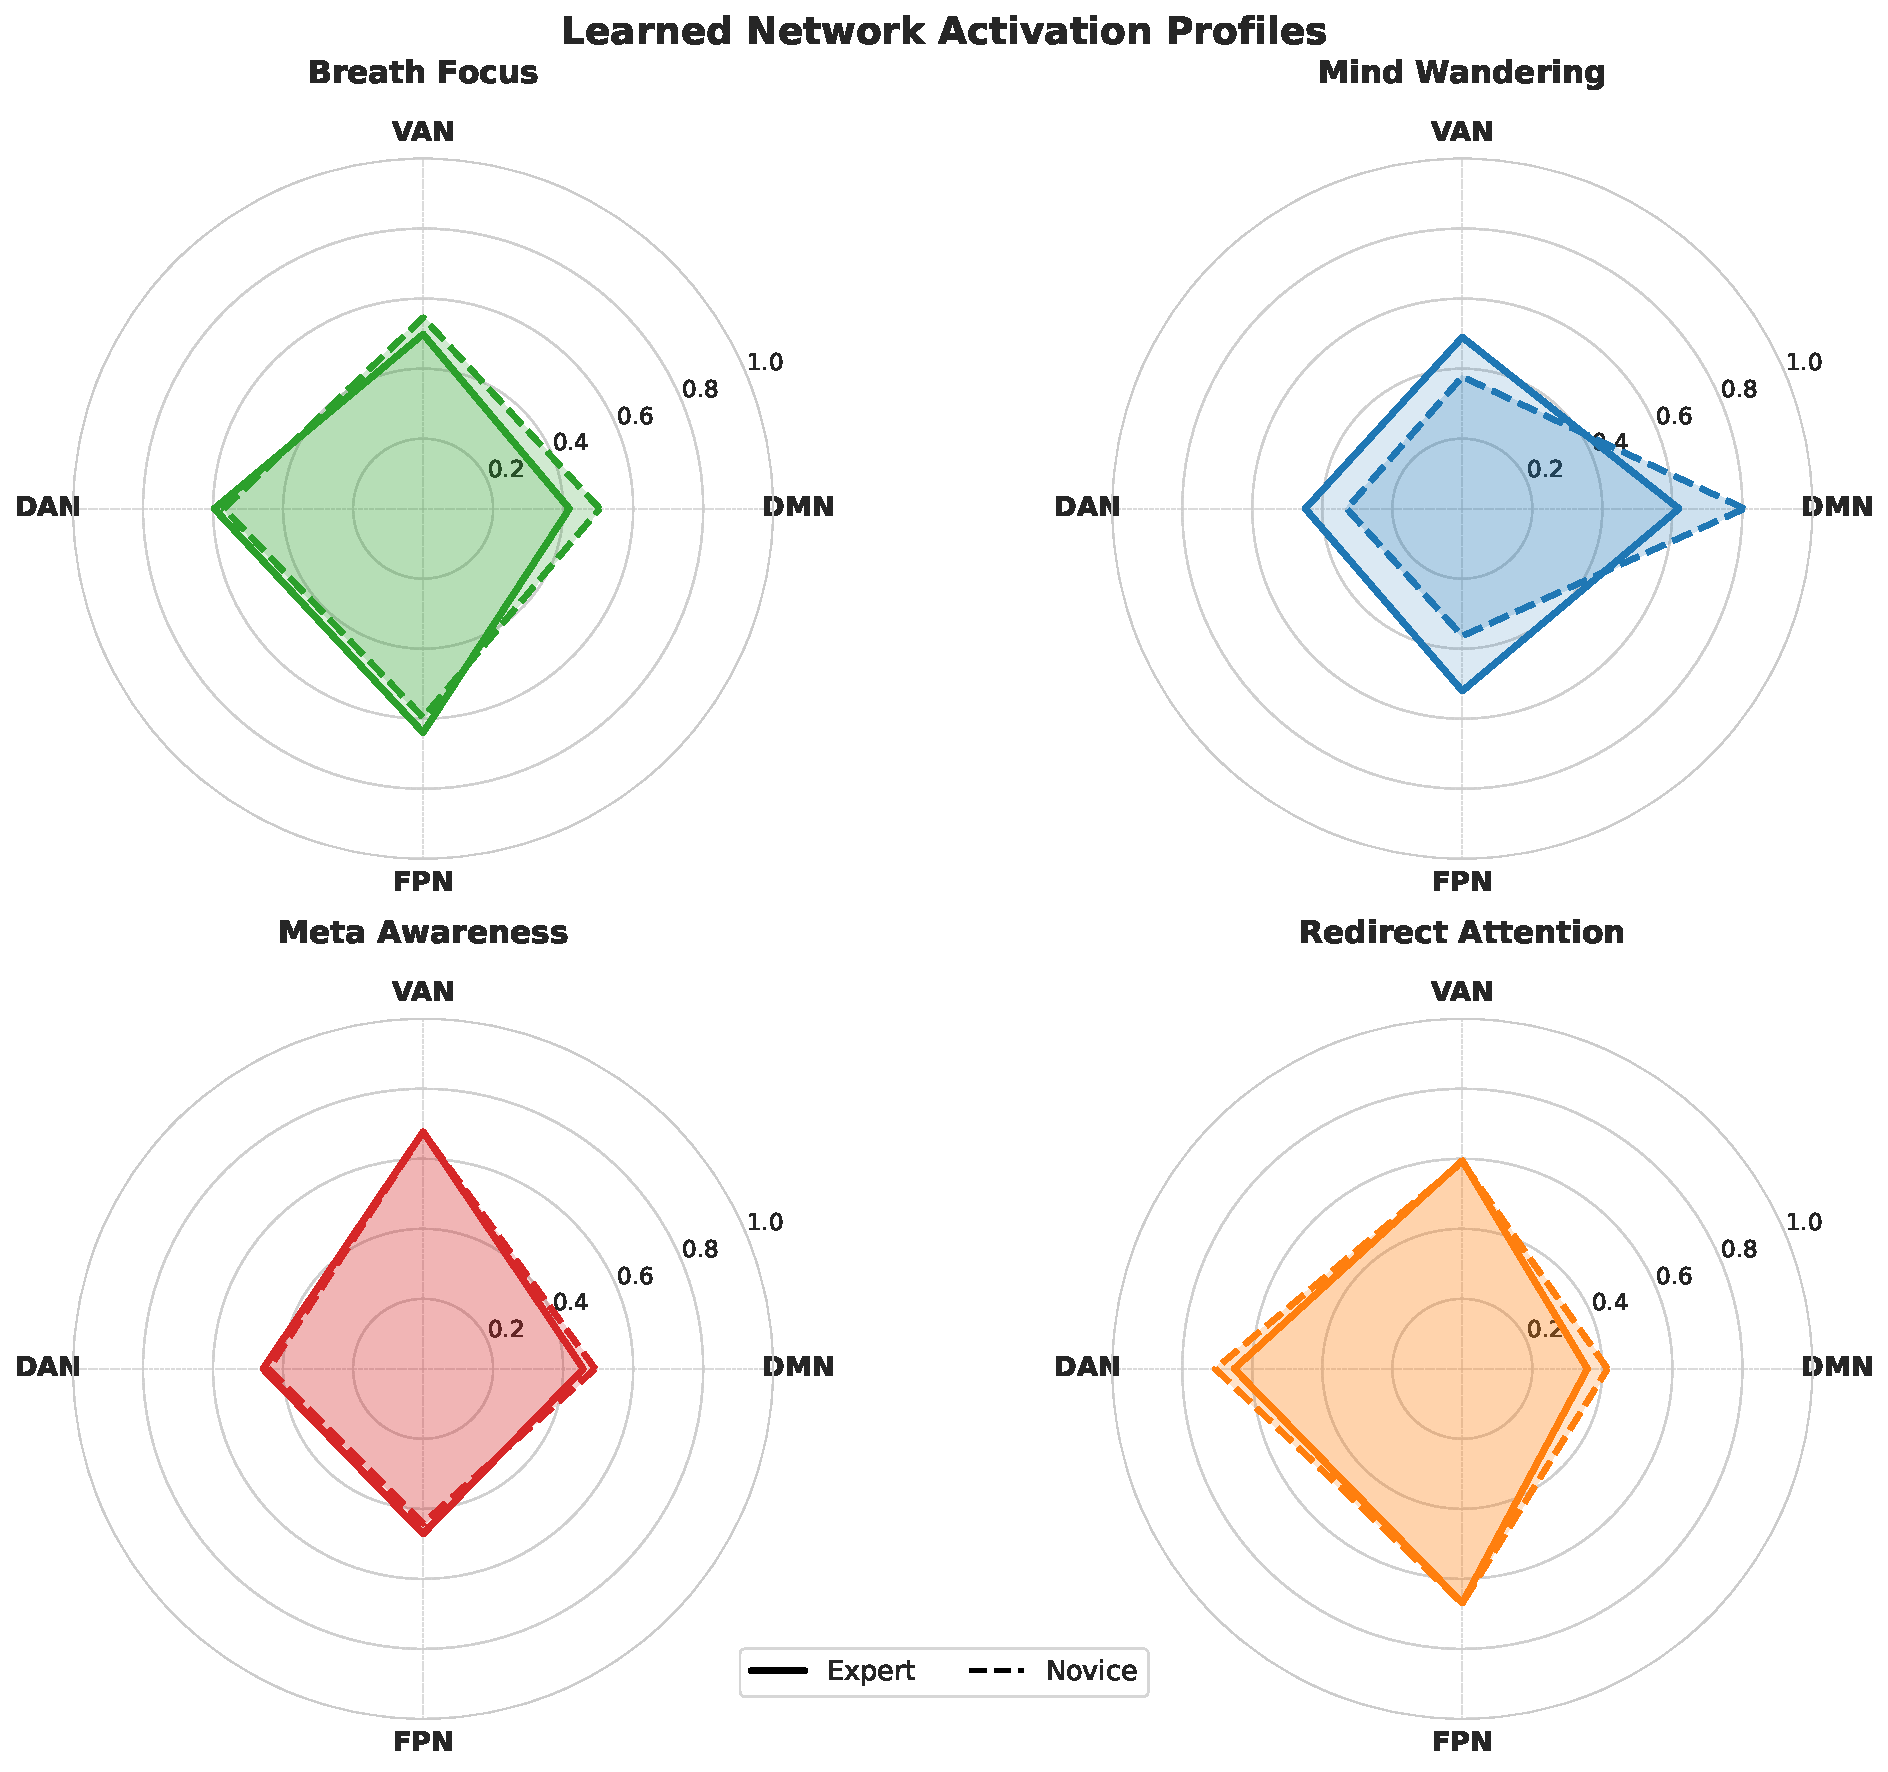
\includegraphics[width=0.9\textwidth]{figures/fig3a.pdf} \\
\small{(A) Novice profile}
\end{tabular}
\vspace{1em}

\begin{tabular}{c}
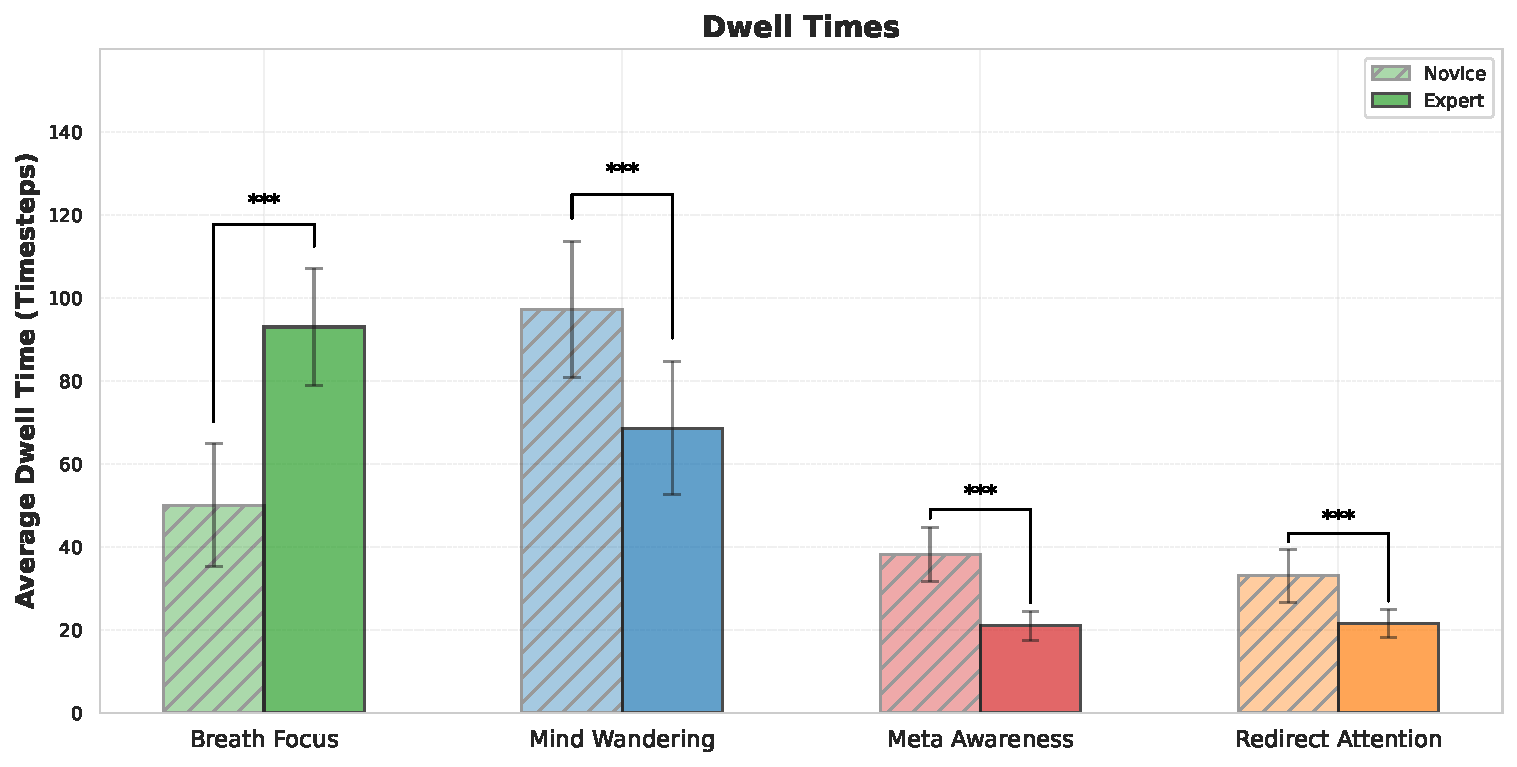
\includegraphics[width=0.9\textwidth]{figures/fig3b.pdf} \\
\small{(B) Expert profile}
\end{tabular}
\caption{\textbf{Hierarchical dynamics.} Across all panels, L3 shows meta-awareness, L2 shows dominant thoughtseeds, and L1 shows network activations (DMN/VAN/DAN/FPN). \textbf{(A) Novice profile.} The novice trace shows higher volatility across levels. State run lengths (from the tail window) show shorter Breath-Focus epochs and prolonged Mind-Wandering: BF $55.0 \pm 12.0$ steps, MW $137.1 \pm 34.0$, MA $38.4 \pm 8.6$. At L2, thoughtseed activations are more diffuse: \textit{attend\_breath} mean $0.36 \pm 0.27$, while \textit{pending\_tasks} $0.38 \pm 0.24$ and \textit{pain\_discomfort} $0.44 \pm 0.23$ are comparatively high. At L1, network activity is DMN-dominant with broader variance: DMN mean $0.65 \pm 0.18$ (range 0.32--0.90), while DAN $0.44 \pm 0.16$ and FPN $0.45 \pm 0.14$ remain lower. DAN--FPN coupling is strong ($r \approx 0.90$), consistent with broad co-activation rather than selective control. Together, these patterns reflect late detection and slow recovery from distraction in the novice simulation. \textbf{(B) Expert profile.} The expert trace shows clearer hierarchical coherence and more stable focus. State run lengths show longer Breath-Focus epochs and shorter Mind-Wandering: BF $86.0 \pm 25.2$, MW $77.7 \pm 15.9$, MA $24.1 \pm 4.6$. At L2, \textit{attend\_breath} is stronger ($0.52 \pm 0.31$) and \textit{pending\_tasks} lower ($0.27 \pm 0.23$), indicating a more focused latent regime. At L1, DMN is lower and less variable ($0.47 \pm 0.13$, range 0.23--0.77) with higher control-network engagement (DAN $0.54 \pm 0.11$, FPN $0.58 \pm 0.09$). DAN--FPN coupling is reduced ($r \approx 0.72$), indicating more selective recruitment. These dynamics reflect sustained focus, faster recovery, and more efficient top-down regulation in the expert simulation.}
\label{fig_3}
\end{figure*}

\subsection{Attractor Dynamics (PCA Trajectories)}

We visualize attractor dynamics using PCA projections of the tail-window trajectories. Instead of free-energy basins, Fig.~\ref{fig_4} emphasizes the geometry and stability of activity in both the low-dimensional thoughtseed space (L2) and the higher-dimensional network space (L1). This highlights the model's central claim: the L2 bottleneck is more tractable and organized, and expertise tightens trajectories in this latent space while reducing diffuseness in network space.

\begin{figure}[!htbp]
    \centering
    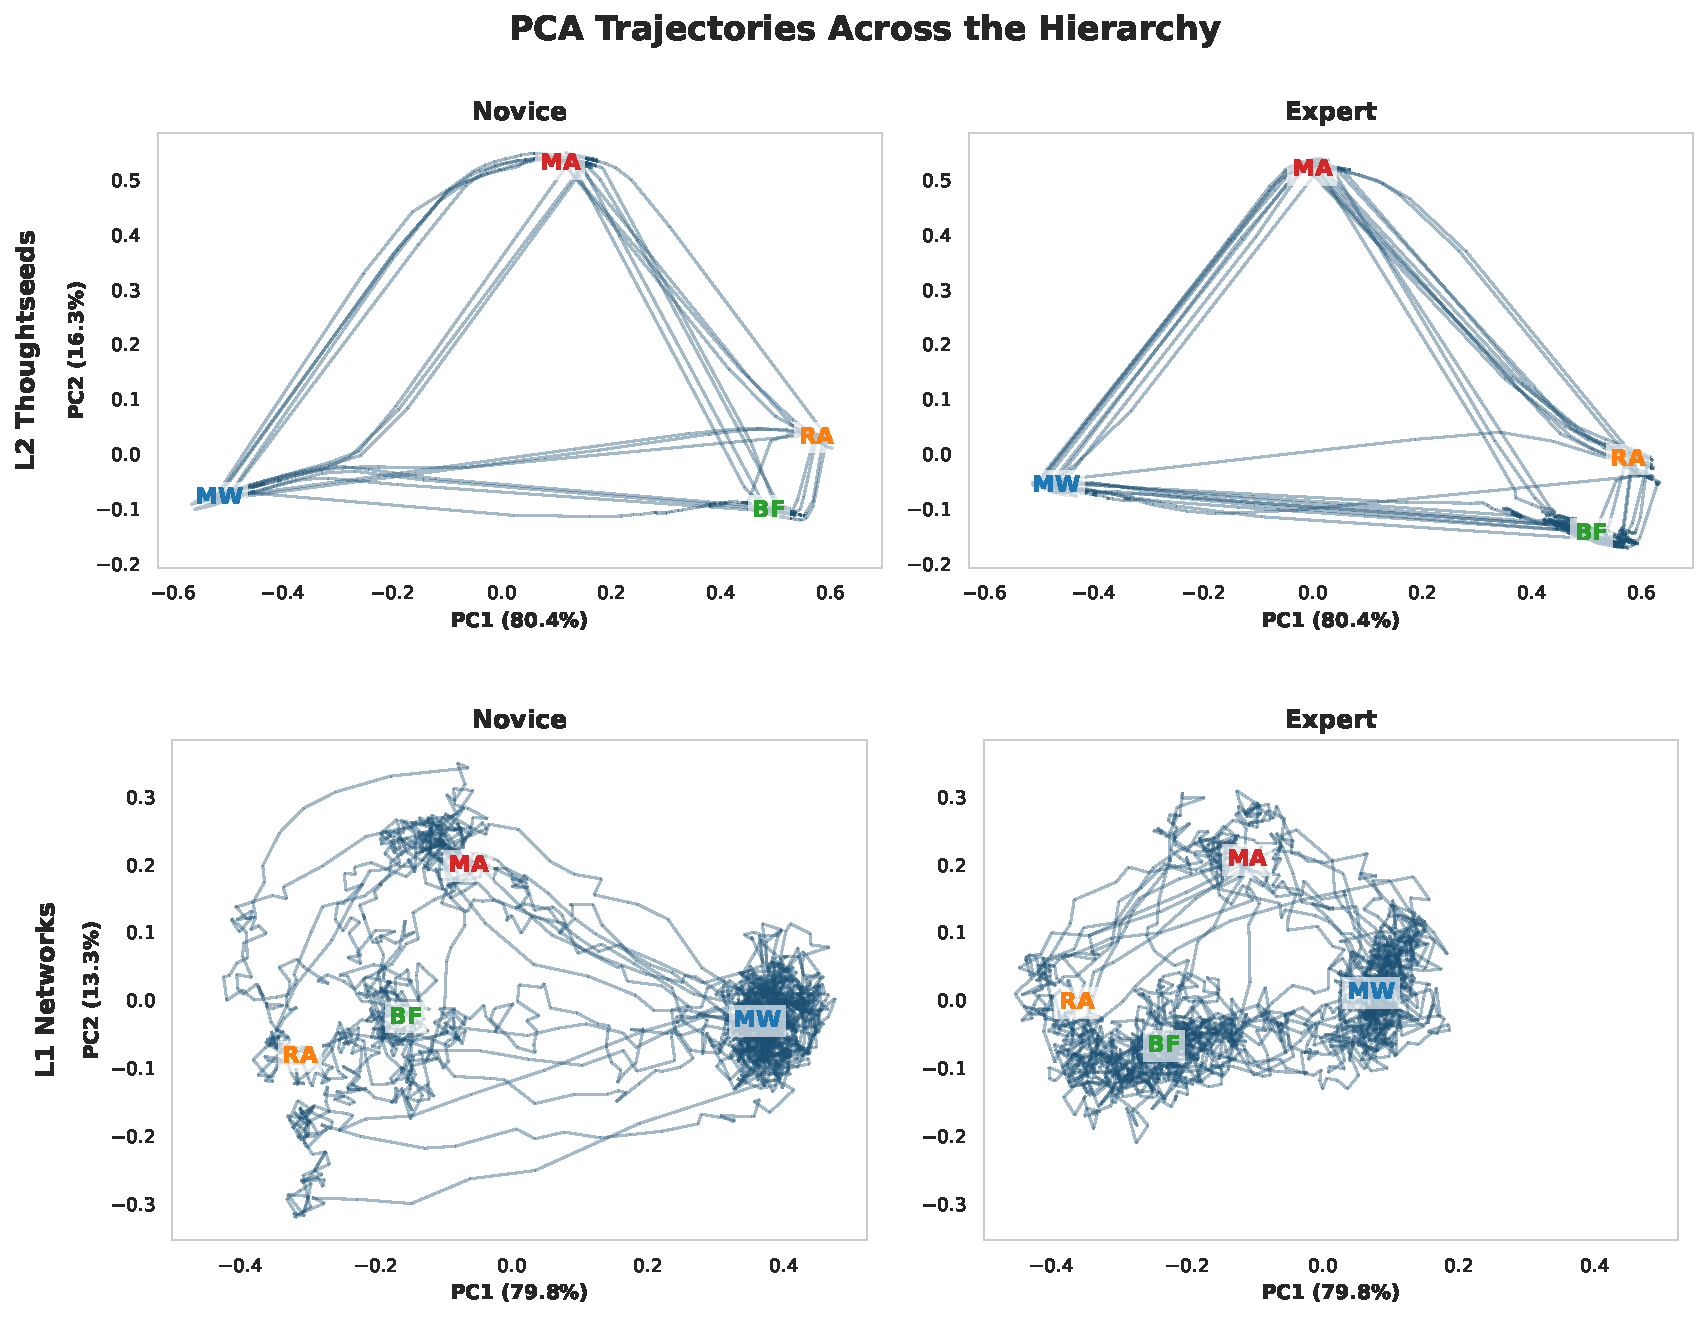
\includegraphics[width=0.95\textwidth]{figures/fig4.pdf}
    \caption{\textbf{PCA Trajectories Across the Hierarchy.} Tail-window trajectories projected using pooled PCA. Top row: L2 thoughtseed trajectories (novice left, expert right; PC1/PC2 explaining 80.4\% and 16.3\% of variance). Bottom row: L1 network trajectories (novice left, expert right; PC1/PC2 explaining 79.8\% and 13.3\%). Expert trajectories are more compact in network space (PC1/PC2 std $\approx$ 0.171/0.102) than novice ($\approx$ 0.281/0.113), indicating tighter attractor dynamics at L1. Thoughtseed dispersion is similar but slightly lower for experts (PC1/PC2 std $\approx$ 0.460/0.206) versus novices ($\approx$ 0.468/0.220), consistent with reduced volatility in the latent bottleneck. The separation between L2 and L1 trajectories underscores the hierarchical architecture: low-dimensional bottleneck dynamics are more orderly and controllable than the underlying network substrate, with expertise tightening trajectories in both spaces while maintaining stronger organization in the thoughtseed layer.}
    \label{fig_4}
\end{figure}

\section{Discussion}

\section{Discussion}

The present work extends the computational phenomenology of mental action in focused-attention meditation \cite{Ramstead2022,SandvedSmith2025}, offering a structured framework that connects first-person experience with quantifiable neural dynamics. Our three-level hierarchy (networks $\rightarrow$ thoughtseeds $\rightarrow$ metacognition) formalizes nested control over attentional contents, in line with predictive-processing theories \cite{LaukkonenSlagter2021} and classical accounts of meditation \cite{Analayo2019}. By anchoring this hierarchy in large-scale brain network organization \cite{Yeo2011} and the Neuronal Packet Hypothesis \cite{Ramstead2021,Yufik2019,YufikFriston2016}, the model proposes a biologically grounded account of competitive interactions among attentional states.

We implement these dynamics using coupled multivariate Ornstein–Uhlenbeck (OU) processes \cite{Gilson2016} and take variational free energy as a functional objective that indexes both inference accuracy and model complexity \cite{ParrPezzuloFriston2022,SandvedSmith2025}. Meditation expertise is modeled via differences in learning rates and phenotype-specific priors (network configurations, dwell-time ranges, transition priors), while precision dynamics emerge from the inference process itself rather than from explicitly stipulated precision parameters. Consistent with contemplative neuroscience, experts show reduced DMN dominance, stronger DAN/FPN engagement, and more stable focus, while novices exhibit more volatile thoughtseed competition and longer mind-wandering episodes \cite{Brewer2011,Seeley2007,Hasenkamp2012}. Experts also show more stable meta-awareness trajectories during mind-wandering and faster redirection, consistent with reports of reduced effort and faster recovery in long-term practitioners \cite{Dahl2015,Fox2015,Tang2015}. These results indicate that bidirectional coupling between latent content (thoughtseeds) and attentional networks captures the integration of top-down and bottom-up processes in meditation \cite{LaukkonenSlagter2021,RaffoneSrinivasan2017}.

\subsection{Limitations and Future Directions}
The current model is a foundational scaffold and does not explicitly distinguish between conscious and unconscious inferential processes. Future extensions could map network dynamics to fast, implicit inference (System‑1‑like) and thoughtseeds to slower, explicit inference (System‑2‑like), consistent with Helmholtzian predictive coding \cite{Clark2013,Hohwy2013,ParrPezzuloFriston2022} and dual‑process accounts \cite{Kahneman2011}. This differentiation also aligns with the Consciousness Prior \cite{Bengio2017}, which motivates discrete attentional agents competing for a capacity‑limited global workspace \cite{Mashour2020,Miller1956}.

Second, the current state‑transition mechanism uses a softmax over Expected Free Energy rather than explicit Bayesian model comparison. Attractor structure emerges from OU processes and single‑step EFE‑based policy selection rather than explicit long‑horizon planning. While our parameter choices (e.g., learning rates, priors) are theoretically motivated, they should be calibrated against empirical measures (e.g., breath‑count accuracy, experience sampling) within neurophenomenological paradigms \cite{Varela2017,Lutz2024}. Network activation targets could also be refined using Hidden Markov Models to infer meditation‑specific hidden states from neuroimaging data.

Furthermore, the current implementation constrains metacognition to modulate L2 precision, while L2 provides the only direct influence on L1 through action‑relevant targets; future versions can further enforce this information bottleneck. A next phase could extend the model to fully autonomous, interacting thoughtseeds, each with its own generative dynamics and precision modulation, enabling emergent coordination through multi‑agent dynamics and dynamic Markov‑blanket detection \cite{BeckRamstead2025}. Incorporating neuromodulatory mechanisms would further strengthen biological plausibility. Beyond meditation, the framework may inform models of attention, mind‑wandering, and meta‑awareness across cognitive domains. 

% (Keep the rest of the rsproca_new template structure as needed:
% sections, equations, figures, tables, conclusions, acknowledgements,
% and references.)
\vspace{\baselineskip}

\ack{We thank the organizers and participants of IWAI 2025 (6th International
Workshop on Active Inference) for comments that helped refine this work from an
initial rules-based approach to a tractable enactive inference implementation,
improving the conceptual architecture, mathematical model, codebase and
manuscript. This research was partially funded by grant PID2021-122136OB-C22,
funded by MICIU/AEI/10.13039/501100011033 and by ERDF ``A way of making
Europe'', and by the AGAUR research support grant 2021 SGR 01035, funded by the
Department of Research and Universities of the Generalitat de Catalunya (G.P.).}

\vspace{\baselineskip}
\noindent\textbf{Author contributions} Conceptualization and methodology: P.C.K.; coding: P.C.K., D.A.F.; writing\textemdash original draft: P.C.K.; writing\textemdash review and editing: P.C.K., D.A.F., G.P.; supervision: G.P.; funding acquisition: G.P. All authors have read and agreed to the current version of the manuscript.

\vspace{\baselineskip}

\noindent\textbf{Disclosure of interests.} The authors declare no conflicts of interest.

\vspace{\baselineskip}

\noindent\textbf{Data Availability Statement}
All simulation code, configuration files, and reference parameters used in this study are openly available in the GitHub repository: \url{https://github.com/prakash-kavi/viapssana_ts2}

\begin{thebibliography}{99}

\bibitem{BrandmeyerDelorme2021}
Brandmeyer T, Delorme A. 2021 Meditation and the wandering mind: a theoretical framework of underlying neurocognitive mechanisms. \textit{Perspect. Psychol. Sci.} \textbf{16}, 39--66. (\href{https://doi.org/10.1177/1745691620917340}{doi:10.1177/1745691620917340})

\bibitem{Tang2015}
Tang YY, H\"olzel BK, Posner MI. 2015 The neuroscience of mindfulness meditation. \textit{Nat. Rev. Neurosci.} \textbf{16}, 213--225. (\href{https://doi.org/10.1038/nrn3916}{doi:10.1038/nrn3916})

\bibitem{Dahl2015}
Dahl CJ, Lutz A, Davidson RJ. 2015 Reconstructing and deconstructing the self: cognitive mechanisms in meditation practice. \textit{Trends Cogn. Sci.} \textbf{19}, 515--523. (\href{https://doi.org/10.1016/j.tics.2015.07.001}{doi:10.1016/j.tics.2015.07.001})

\bibitem{Fox2014}
Fox KCR, Nijeboer S, Dixon ML, Floman JL, Ellamil M, Rumak SP \textit{et al.} 2014 Is meditation associated with altered brain structure? A systematic review and meta-analysis of morphometric neuroimaging in meditation practitioners. \textit{Neurosci. Biobehav. Rev.} \textbf{43}, 48--73. (\href{https://doi.org/10.1016/j.neubiorev.2014.03.016}{doi:10.1016/j.neubiorev.2014.03.016})

\bibitem{Analayo2019}
An\=alayo B. 2019 \textit{Satipa\d{t}\d{t}h\=ana meditation: a practice guide}. Cambridge, UK: Windhorse Publications.

\bibitem{Hasenkamp2012}
Hasenkamp W, Wilson-Mendenhall CD, Duncan E, Barsalou LW. 2012 Mind wandering and attention during focused meditation: a fine-grained temporal analysis of fluctuating cognitive states. \textit{Neuroimage} \textbf{59}, 750--760. (\href{https://doi.org/10.1016/j.neuroimage.2011.07.008}{doi:10.1016/j.neuroimage.2011.07.008})

\bibitem{Lutz2008}
Lutz A, Slagter HA, Dunne JD, Davidson RJ. 2008. Attention regulation and monitoring in meditation. \textit{Trends Cogn Sci} \textbf{12}, 163--169. (\href{https://doi.org/10.1016/j.tics.2008.01.005}{doi:10.1016/j.tics.2008.01.005})

\bibitem{ZamoraLopez2016}
Zamora-Lopez G, Chen Y, Deco G, Kringelbach ML, Zhou C. 2016. Functional complexity emerging from anatomical constraints in the brain: The significance of network modularity and rich-clubs. \textit{Sci Rep} \textbf{6}, 38424. (\href{https://doi.org/10.1038/srep38424}{doi:10.1038/srep38424})

\bibitem{BarrettSimmons2015}
Barrett LF, Simmons WK. 2015. Interoceptive predictions in the brain. \textit{Nat Rev Neurosci} \textbf{16}, 419--429. (\href{https://doi.org/10.1038/nrn3950}{doi:10.1038/nrn3950})

\bibitem{LaukkonenSlagter2021}
Laukkonen RE, Slagter HA. 2021. From many to one: The science of consciousness and the contemplative path to nondual awakening. \textit{Prog Brain Res} \textbf{258}, 227--259.

\bibitem{Friston2010}
Friston K. 2010 The free-energy principle: A unified brain theory?
\textit{Nat. Rev. Neurosci.} \textbf{11}, 127--138. (\href{https://doi.org/10.1038/nrn2787}{doi:10.1038/nrn2787})

\bibitem{ParrFriston2018}
Parr T, Friston KJ. 2018 The active construction of conscious experience.
\textit{Neurosci. Conscious.} 2018:niy015. (\href{https://doi.org/10.1093/nc/niy015}{doi:10.1093/nc/niy015})

\bibitem{Kirchhoff2018}
Kirchhoff M, Parr T, Palacios E, Friston K, Kiverstein J. 2018 The Markov
blankets of life: Autonomy, active inference and the free energy principle.
\textit{J. R. Soc. Interface} \textbf{15}, 20170792.
(\href{https://doi.org/10.1098/rsif.2017.0792}{doi:10.1098/rsif.2017.0792})

\bibitem{Friston2017}
Friston KJ, FitzGerald T, Rigoli F, Schwartenbeck P, Pezzulo G. 2017. Active inference: A process theory. \textit{Neural Computation} \textbf{29}, 1--49. (\href{https://doi.org/10.1162/NECO_a_00912}{doi:10.1162/NECO\_a\_00912})

\bibitem{Ramstead2020}
Ramstead MJD, Kirchhoff MD, Friston KJ. 2020. A tale of two densities: Active inference is enactive inference. \textit{Adaptive Behavior} \textbf{28}, 225--239. (\href{https://doi.org/10.1177/1059712319862774}{doi:10.1177/1059712319862774})

\bibitem{Yufik2019}
Yufik YM. 2019. The understanding capacity and information dynamics in the human brain. \textit{Entropy} \textbf{21}, 308. (\href{https://doi.org/10.3390/e21030308}{doi:10.3390/e21030308})

\bibitem{YufikFriston2016}
Yufik YM, Friston KJ. 2016. Life and understanding: The origins of `understanding' in self-organizing nervous systems. \textit{Frontiers in Systems Neuroscience} \textbf{10}, 98. (\href{https://doi.org/10.3389/fnsys.2016.00098}{doi:10.3389/fnsys.2016.00098})

\bibitem{Ramstead2021}
Ramstead MJD, Hesp C, Tschantz A, Smith R, Constant A, Friston KJ. 2021. Neural and phenotypic representation under the free-energy principle. \textit{Neuroscience and Biobehavioral Reviews} \textbf{120}, 109--122. (\href{https://doi.org/10.1016/j.neubiorev.2020.11.024}{doi:10.1016/j.neubiorev.2020.11.024})

\bibitem{SpornsBetzel2016}
Sporns O, Betzel RF. 2016. Modular brain networks. \textit{Annual Review of Psychology} \textbf{67}, 613--640. (\href{https://doi.org/10.1146/annurev-psych-122414-033634}{doi:10.1146/annurev-psych-122414-033634})

\bibitem{Hipolito2021}
Hipólito I, Ramstead MJD, Convertino L, Bhat A, Friston K, Parr T. 2021. Markov blankets in the brain. \textit{Neurosci Biobehav Rev} 125, 88--97. (\href{https://doi.org/10.1016/j.neubiorev.2021.02.003}{doi:10.1016/j.neubiorev.2021.02.003})

\bibitem{Ramstead2022}
Ramstead MJD, Seth AK, Hesp C, Sandved-Smith L, Mago J, Lifshitz M, et al. 2022. From generative models to generative passages: A computational approach to (neuro)phenomenology. \textit{Rev Philos Psychol} 13, 829--857. (\href{https://doi.org/10.1007/s13164-021-00604-y}{doi:10.1007/s13164-021-00604-y})

\bibitem{Palacios2020}
Palacios ER, Razi A, Parr T, Kirchhoff M, Friston K. 2020. On Markov blankets and hierarchical self-organisation. \textit{J Theor Biol} 486, 110089. (\href{https://doi.org/10.1016/j.jtbi.2019.110089}{doi:10.1016/j.jtbi.2019.110089})

\bibitem{Czajko2024}
Czajko S, Zorn J, Daumail L, Chetelat G, Margulies DS, Lutz A. 2024. Exploring the embodied mind: Functional connectome fingerprinting of meditation expertise. \textit{Biol Psychiatry Glob Open Sci} 4, 100372. (\href{https://doi.org/10.1016/j.bpsgos.2024.100372}{doi:10.1016/j.bpsgos.2024.100372})

\bibitem{Hohwy2013}
Hohwy J. 2013. \textit{The Predictive Mind}. Oxford, UK: Oxford University Press. (\href{https://doi.org/10.1093/acprof:oso/9780199682737.001.0001}{doi:10.1093/acprof:oso/9780199682737.001.0001})

\bibitem{Varela2017}
Varela FJ, Thompson E, Rosch E. 2017. The embodied mind: cognitive science and human experience. Cambridge, MA: MIT Press. (\href{https://doi.org/10.7551/mitpress/9780262529365.001.0001}{doi:10.7551/mitpress/9780262529365.001.0001})

\bibitem{Kavi2025}
Kavi PC, Zamora-L\'opez G, Friedman DA, Patow G. 2025. Thoughtseeds: a hierarchical and agentic framework for investigating thought dynamics in meditative states. Entropy \textbf{27}, 459. (\href{https://doi.org/10.3390/e27050459}{doi:10.3390/e27050459})

\bibitem{Bengio2017}
Bengio Y. 2017. The consciousness prior. arXiv. (\href{https://doi.org/10.48550/arXiv.1709.08568}{doi:10.48550/arXiv.1709.08568})

\bibitem{Mashour2020}
Mashour GA, Roelfsema PR, Changeux J-P, Dehaene S. 2020. Conscious processing and the global neuronal workspace hypothesis. Neuron \textbf{105}, 776--798. (\href{https://doi.org/10.1016/j.neuron.2020.01.026}{doi:10.1016/j.neuron.2020.11.026})

\bibitem{DehaeneChangeux2011}
Dehaene S, Changeux J-P. 2011 Experimental and theoretical approaches to conscious processing. \textit{Neuron} \textbf{70}, 200--227. (\href{https://doi.org/10.1016/j.neuron.2011.03.018}{doi:10.1016/j.neuron.2011.03.018})

\bibitem{Safron2020}
Safron A. 2020 An integrated world modeling theory (IWMT) of consciousness: combining integrated information and global neuronal workspace theories with the free energy principle and active inference. \textit{Entropy} \textbf{22}, 646. (\href{https://doi.org/10.3390/e22060646}{doi:10.3390/e22060646})

\bibitem{Yeo2011}
Yeo BTT, Krienen FM, Sepulcre J, Sabuncu MR, Lashkari D, Hollinshead M \textit{et al.} 2011 The organization of the human cerebral cortex estimated by intrinsic functional connectivity. \textit{J. Neurophysiol.} \textbf{106}, 1125--1165. (\href{https://doi.org/10.1152/jn.00338.2011}{doi:10.1152/jn.00338.2011})

\bibitem{SandvedSmith2025}
Sandved-Smith L, Bogotá JD, Hohwy J, Kiverstein J, Lutz A. 2025 Deep computational neurophenomenology: a methodological framework for investigating the how of experience. \textit{Neurosci. Conscious.} \textbf{2025}, niaf016. (\href{https://doi.org/10.1093/nc/niaf016}{doi:10.1093/nc/niaf016})

\bibitem{Fox2015}
Fox KCR, Spreng RN, Ellamil M, Andrews-Hanna JR, Christoff K. 2015 The wandering brain: meta-analysis of functional neuroimaging studies of mind-wandering and related spontaneous thought processes. \textit{Neuroimage} \textbf{111}, 611--621. (\href{https://doi.org/10.1016/j.neuroimage.2015.02.039}{doi:10.1016/j.neuroimage.2015.02.039})

\bibitem{Brewer2011}
Brewer, J. A., Worhunsky, P. D., Gray, J. R., Tang, Y.-Y., Weber, J.\ and Kober, H.\ 2011 Meditation experience is associated with differences in default mode network activity and connectivity. \textit{Proc. Natl Acad. Sci. USA} \textbf{108}, 20\,254--20\,259. (\href{https://doi.org/10.1073/pnas.1112029108}{doi:10.1073/pnas.1112029108})

\bibitem{Friston2014}
Friston, K., Sengupta, B.\ and Auletta, G.\ 2014 Cognitive dynamics: from attractors to active inference. \textit{Proc. IEEE} \textbf{102}, 427--445. (\href{https://doi.org/10.1109/JPROC.2014.2306251}{doi:10.1109/JPROC.2014.2306251})

\bibitem{Ramstead2023}
Ramstead, M., Albarracin, M., Kiefer, A., Klein, B., Fields, C., Friston, K.\ and Safron, A.\ 2023 The inner screen model of consciousness: applying the free energy principle directly to the study of conscious experience. \textit{arXiv} 2305.02205.

\bibitem{Gilson2016}
Gilson, M., Moreno-Bote, R., Ponce-Alvarez, A., Ritter, P.\ and Deco, G.\ 2016 Estimation of directed effective connectivity from fMRI functional connectivity hints at asymmetries of cortical connectome. \textit{PLoS Comput. Biol.} \textbf{12}, e1004762. (\href{https://doi.org/10.1371/journal.pcbi.1004762}{doi:10.1371/journal.pcbi.1004762})

\bibitem{KingmaWelling2013}
Kingma, D. P.\ and Welling, M.\ 2013 Auto-encoding variational Bayes. \textit{arXiv} 1312.6114.

\bibitem{Miller1956}
Miller GA. 1956. The magical number seven, plus or minus two: some limits on our capacity for processing information. Psychol. Rev. 63, 81--97. (\href{https://doi.org/10.1037/h0043158}{doi:10.1037/h0043158})

\bibitem{MacLean2010}
MacLean KA, Ferrer E, Aichele SR, Bridwell DA, Zanesco AP, Jacobs TL et al. 2010. Intensive meditation training improves perceptual discrimination and sustained attention. Psychol. Sci. 21, 829--839. (\href{https://doi.org/10.1177/0956797610371339}{doi:10.1177/0956797610371339})

\bibitem{Seeley2007}
Seeley WW, Menon V, Schatzberg AF, Keller J, Glover GH, Kenna H et al. 2007. Dissociable intrinsic connectivity networks for salience processing and executive control. J. Neurosci. 27, 2349--2356. (\href{https://doi.org/10.1523/JNEUROSCI.5587-06.2007}{doi:10.1523/JNEUROSCI.5587-06.2007})

\bibitem{Escrichs2019}
Escrichs A, Sanju\'an A, Atasoy S, L\'opez-Gonz\'alez A, Garrido C, C\`amara E et al. 2019. Characterizing the dynamical complexity underlying meditation. Front. Syst. Neurosci. 13, 27. (\href{https://doi.org/10.3389/fnsys.2019.00027}{doi:10.3389/fnsys.2019.00027})

\bibitem{Christoff2009}
Christoff K, Gordon AM, Smallwood J, Smith R, Schooler JW. 2009. Experience sampling during fMRI reveals default network and executive system contributions to mind wandering. Proc. Natl Acad. Sci. USA 106, 8719--8724. (\href{https://doi.org/10.1073/pnas.0900234106}{doi:10.1073/pnas.0900234106})

\bibitem{Lutz2024}
Lutz A, Abdoun O, Dor-Ziderman Y, Trautwein FM, Berkovich-Ohana A. 2024. An overview of neurophenomenological approaches to meditation and their relevance to clinical research. Biol. Psychiatry Cogn. Neurosci. Neuroimaging 10, 411--424. (\href{https://doi.org/10.1016/j.bpsc.2024.11.008}{doi:10.1016/j.bpsc.2024.11.008})

\bibitem{Schooler2011}
Schooler JW, Smallwood J, Christoff K, Handy TC, Reichle ED, Sayette MA. 2011. Meta-awareness, perceptual decoupling and the wandering mind. Trends Cogn. Sci. 15, 319--326. (\href{https://doi.org/10.1016/j.tics.2011.05.006}{doi:10.1016/j.tics.2011.05.006})

\bibitem{Analayo2021}
An\=alayo B. 2021. Dependent arising and interdependence. \textit{Mindfulness} \textbf{12}, 1094--1102. (\href{https://doi.org/10.1007/s12671-020-01544-x}{doi:10.1007/s12671-020-01544-x})

\bibitem{RaffoneSrinivasan2017}
Raffone A, Srinivasan N. 2017. Mindfulness and cognitive functions: Toward a unifying neurocognitive framework. \textit{Mindfulness} \textbf{8}, 1--9. (\href{https://doi.org/10.1007/s12671-016-0654-1}{doi:10.1007/s12671-016-0654-1})

\bibitem{Clark2013}
Clark A. 2013. Whatever next? Predictive brains, situated agents, and the future of cognitive science. \textit{Behav. Brain Sci.} \textbf{36}(3), 181--204. (\href{https://doi.org/10.1017/S0140525X12000477}{doi:10.1017/S0140525X12000477})

\bibitem{ParrPezzuloFriston2022}
Parr T, Pezzulo G, Friston KJ. 2022. \textit{Active Inference: The Free Energy Principle in Mind, Brain, and Behavior}. Cambridge, MA: MIT Press. (\href{https://doi.org/10.7551/mitpress/12441.001.0001}{doi:10.7551/mitpress/12441.001.0001})

\bibitem{Kahneman2011}
Kahneman D. 2011. \textit{Thinking, fast and slow}. New York, NY: Farrar, Straus and Giroux.

\bibitem{BeckRamstead2025}
Beck J, Ramstead MJD. 2025. Dynamic Markov Blanket Detection for Macroscopic Physics Discovery. \textit{arXiv} [Preprint] arXiv:2502.21217. (\href{https://doi.org/10.48550/arXiv.2502.21217}{doi:10.48550/arXiv.2502.21217})

\bibitem{DecoJirsa2012}
Deco G, Jirsa VK. 2012. Ongoing cortical activity at rest: Criticality, multistability, and ghost attractors. \textit{J. Neurosci.} \textbf{32}, 3366--3375. (\href{https://doi.org/10.1523/JNEUROSCI.2523-11.2012}{doi:10.1523/JNEUROSCI.2523-11.2012})

\bibitem{Deco2021}
Deco G, Vidaurre D, Kringelbach ML. 2021. Revisiting the global workspace orchestrating the hierarchical organization of the human brain. \textit{Nat. Hum. Behav.} \textbf{5}, 497--511. (\href{https://doi.org/10.1038/s41562-020-01003-6}{doi:10.1038/s41562-020-01003-6})
\end{thebibliography}

\end{document}
